\chapter{The ATLAS experiment}

\label{ch:atlas}
\par ATLAS (A Toroidal LHC ApparatuS) is one of the major experiments located at Point 1 of the Large Hadron Collider (LHC) at CERN. 
It is a general-purpose particle physics experiment, which is designed to exploit the huge range of physics opportunities that the LHC provides. 
		Located at 92 m below ground, ATLAS has a cylinder shape which has a length of  46 m, a diameter of 25 m and a weight of over 7000 tons.
 The experiment is a collaboration involving roughly 3,000 physicists from over 175 institutions in 38 countries\cite{fact}.
A right-handed Cartesian coordinate system is used in this thesis: the coordinate origin is at the geometric center of the ATLAS detector, with a z-axis as 
the direction of beam pipe.
\par The x-y plane is perpendicular to the z-axis, with x pointing from origin point to the center 
of LHC ring and y pointing upward. Therefore, polar angle $\theta$ is measured with respect to z-axis and azimuthal angle $\phi$ is measured around the beam axis. 
\par The pseudorapidity is defined as $\eta = ln~tan(\frac{\theta}{2})$. The distance $\Delta R$ in the pseudorapidity-azimuthal plane is defined as 
$\Delta R = \sqrt{\Delta\eta^2 + \Delta\phi^2}$. Transverse momentum $P_T$, transverse energy $E_T$ and missing transverse energy $E_T^{miss}$ are all defined in x-y plane.				

\begin{figure}[htbp]
  \begin{center}
    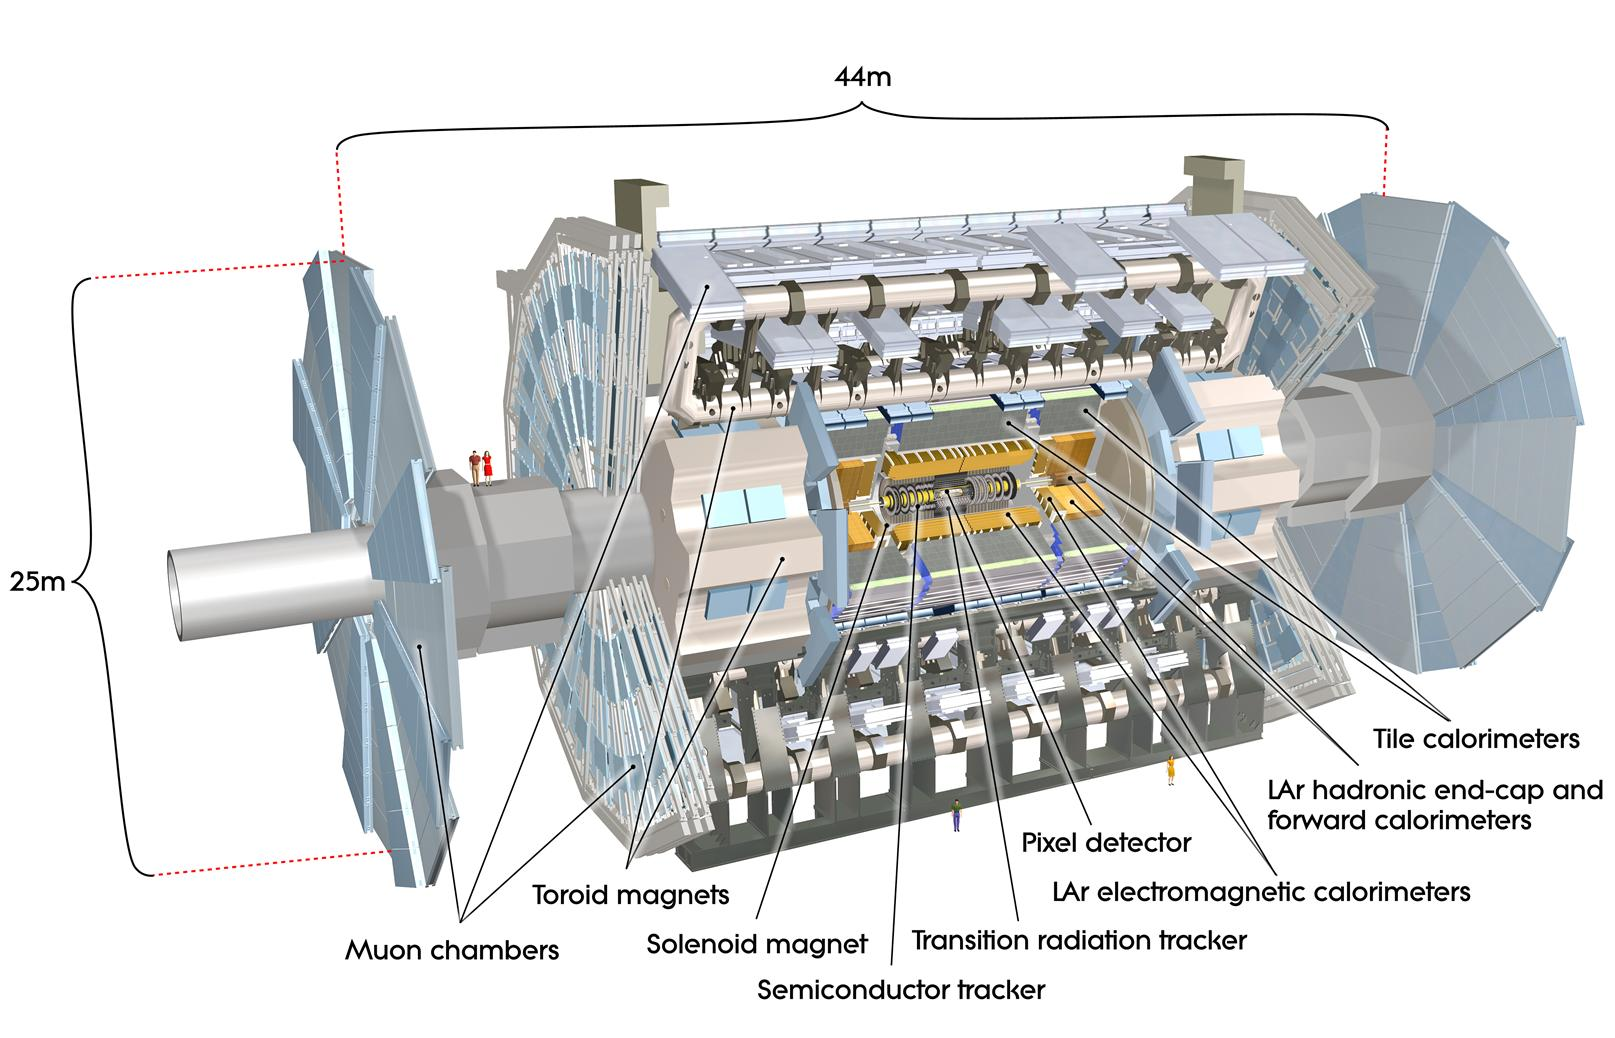
\includegraphics[width=0.8\textwidth]{chapters/c4/figures/atlas.jpg}
  \end{center}
  \caption{Cut-away view of the ATLAS detector}
  \label{fig:cutaway}
\end{figure}
A cut-away view of ATLAS detector is showed in Fig~\ref{fig:cutaway}. 
\par The four major components of the ATLAS detector are the Inner Detector, the Calorimeter, the Muon Spectrometer,
 and the Magnet System. Integrated with the detector components are: the Trigger and Data Acquisition System, 
a specialized multi-level computing system, which selects physics events with distinguishing characteristics; 
and the Computing System, which develops and improves computing software used to store, process and analyze vast amounts of collision data 
at 130 computing centers worldwide\cite{atlas}.
\begin{figure}[htbp]
  \begin{center}
    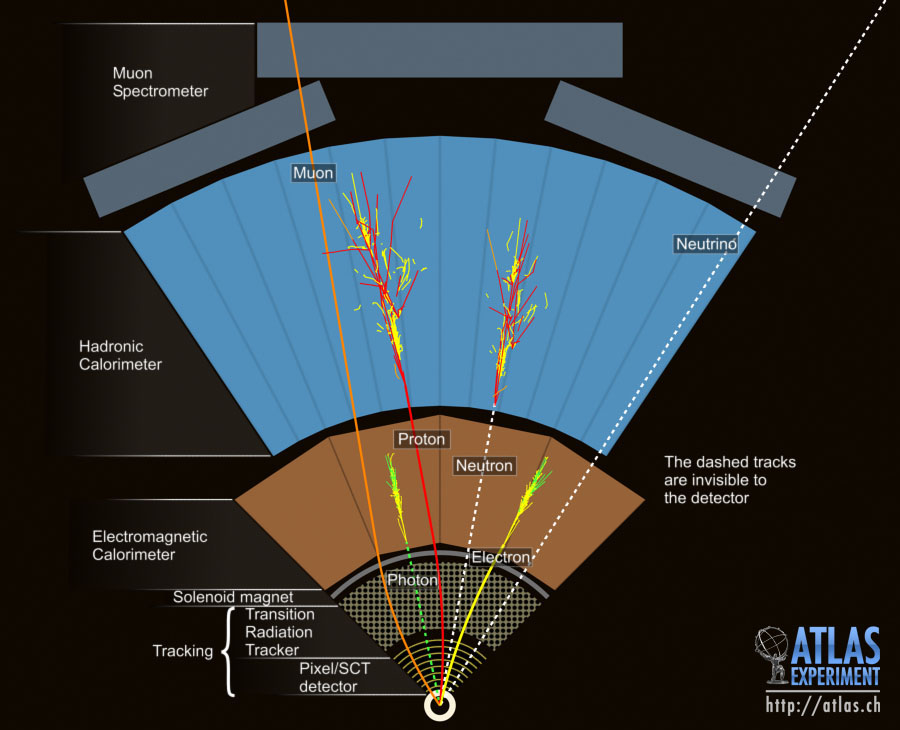
\includegraphics[width=0.8\textwidth]{chapters/c4/figures/eve_gen.jpg}
  \end{center}
  \caption{A computer-generated image of
the ATLAS detector, showing the
different layers and the passage
of different particle types through
the layers.}
  \label{fig:eve-gen}
\end{figure}
\par Different particles leave their passage in different layers in Fig~\ref{fig:eve-gen}, where Pixel and SCT Tracker store $\frac{q}{p_T}$ (charge over transverse momentum), the measurement of charged particles, Calorimeters measure energy measurement of electromagnetically and hadronically interacting particles, and Muon Spectrometer measure additional tracker for muons.		 	 	 		
\par This chapter is intended as a brief introduction to the ATLAS sub-systems,
 including Inner detector in Section~\ref{sec:inner}, calorimeters in Section~\ref{sec:calo}, 
muon system in Section~\ref{sec:muon}, Forward detectors in Section~\ref{sec:for}, and trigger and data acquisition system in Section~\ref{sec:data}.


\section{Inner detector}
\label{sec:inner}
\begin{figure}[htbp]
  \begin{center}
    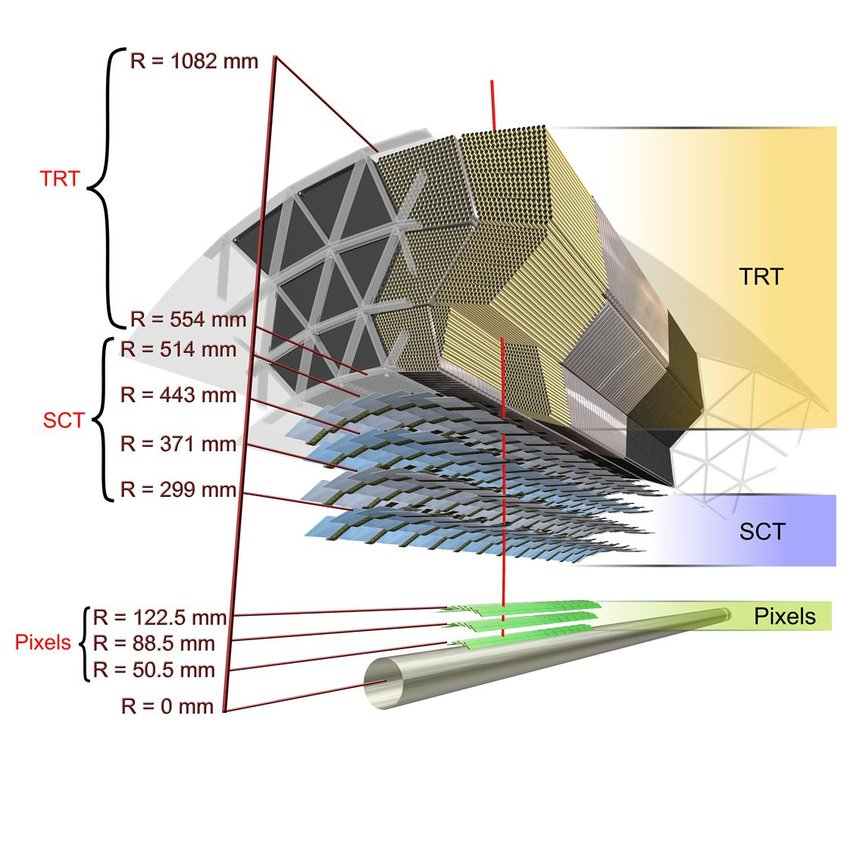
\includegraphics[width=0.8\textwidth]{chapters/c4/figures/inner}
  \end{center}
    \caption{Cut-away view of the ATLAS Inner Detector.}
  \label{fig:inner}
\end{figure}
\par The Inner Detector tracker is important for track reconstruction as well as both primary and secondary vertex measurements for charged tracks in the pseudorapidity range of $ \eta< 2.5$. 
The Inner Detector tracker is contained within a cylindrical envelope with a length of $\pm$3512 mm, a radius of 1150 mm.
\par As shown in Fig~\ref{fig:inner}, the Inner Detector tracker comprises three detector types dedicated to tracking, moving inside out we find the Silicon Pixel Detector, the SemiConductor Tracker (SCT), and the Transition Radiation Tracker (TRT). An extra pixel detector layer (IBL)\cite{Capeans:1291633} was inserted before the Run 2 and improves the identification of b-jets\cite{ATL-PHYS-PUB-2015-022}. The Pixel system provides a coverage of $|\eta|<2.5$.
The SCT system consists of four barrel double layers and 18 end-cap layers (9 on each end)\cite{Aad:2014mta}, and provides a coverage of $|\eta| < 2.5$.
The TRT consists of 70 barrel layers and 280 end-cap layers (140 on each end), and provides a coverage of $|\eta| < 2.0$\cite{Aad:2014mta}.


\subsection{Pixel detector}
\label{sec:pixel}


\begin{figure}
\begin{subfigure}{.5\textwidth}
  \centering
    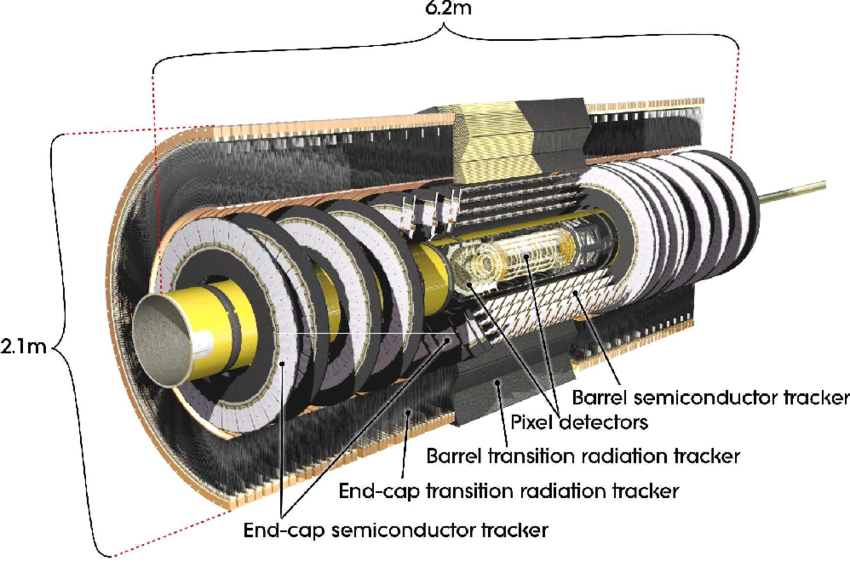
\includegraphics[width=0.8\textwidth]{chapters/c4/figures/pixel}
  \caption{a}
  \label{fig:pixel1}
\end{subfigure}%
\begin{subfigure}{.5\textwidth}
  \centering
    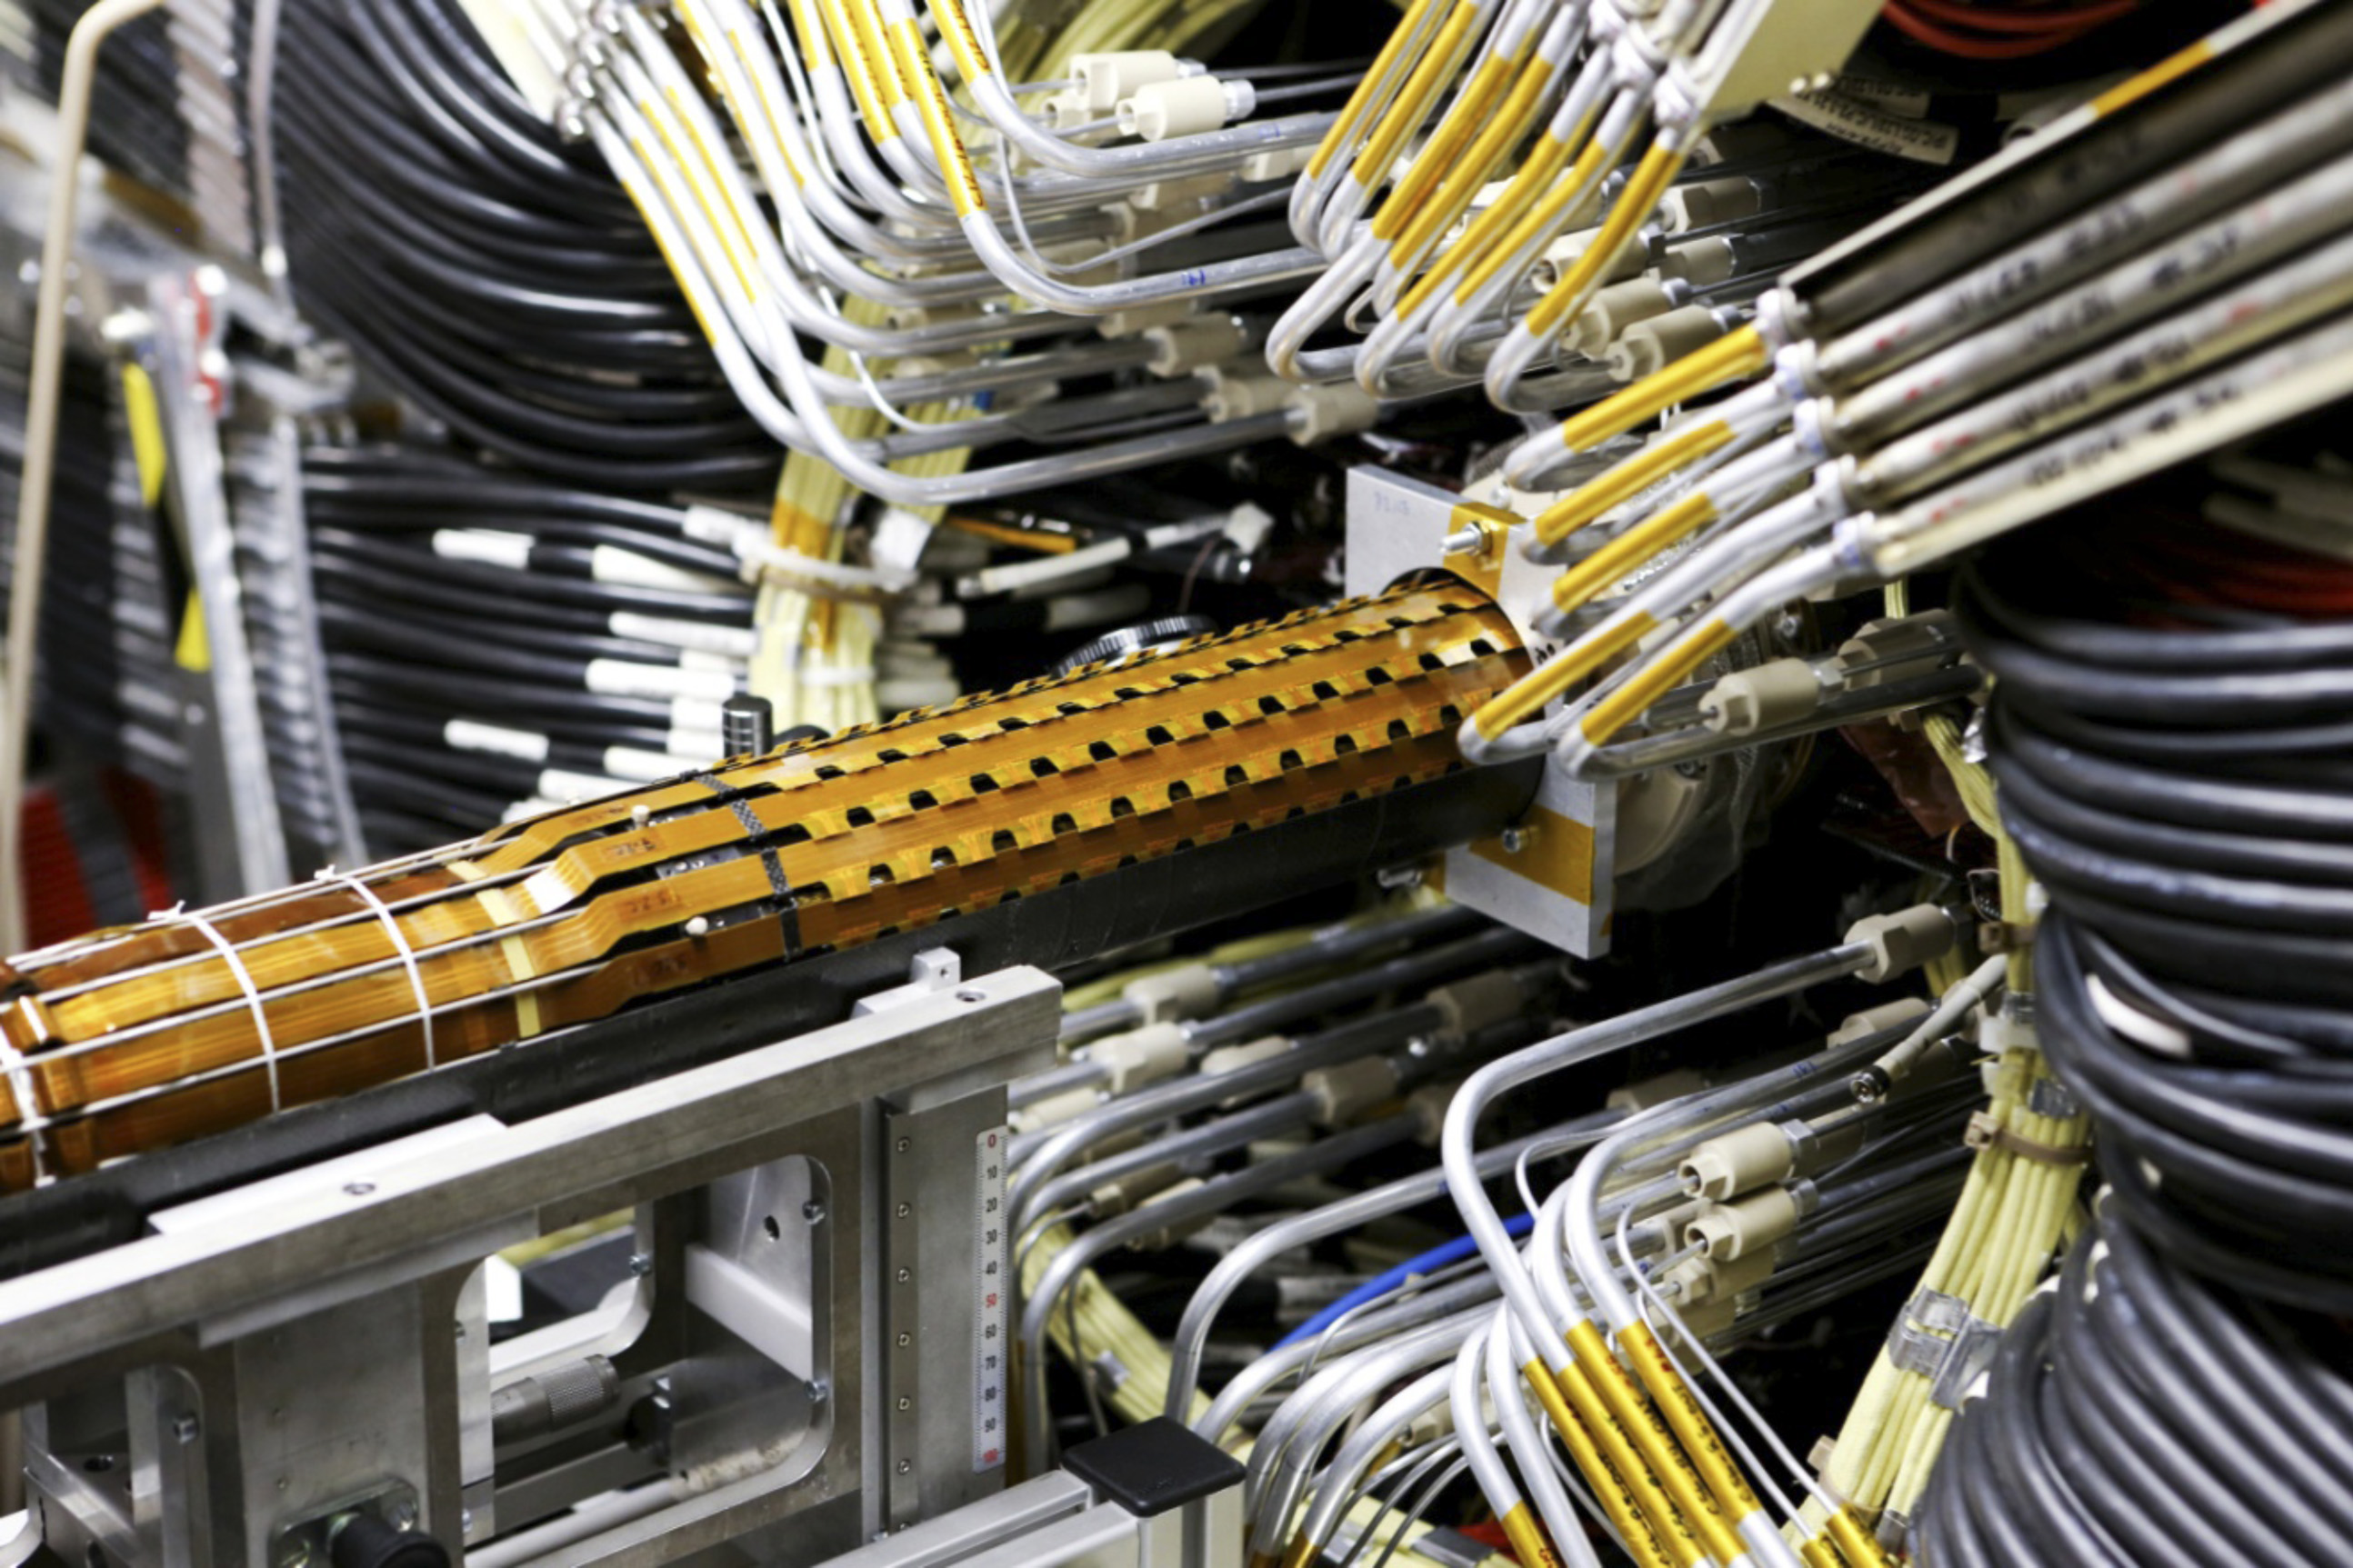
\includegraphics[width=0.8\textwidth]{chapters/c4/figures/IBL}
  \caption{b}
  \label{fig:pixel2}
\end{subfigure}
    \caption{A schematic view of the active region of the Pixel detector consisting of barrel and endcap layers (\ref{fig:pixel1}) and IBL detector before the insertion (\ref{fig:pixel2})}
\label{fig:pixel}
\end{figure}
\par  With the fine granularity of the pixel sensors, the pixel detector is designed to provide the identification and reconstruction of secondary vertices from the long-lived particles and high resolution for primary vertices reconstruction to suppress pile-up due to the increase of luminosity for LHC. A schematic view of the active region of the pixel detector consisting of a barrel and endcap layers can be found in Fig~\ref{fig:pixel1}.
\par  With the fine granularity of the pixel sensors, the pixel detector is designed to provide the identification and reconstruction of secondary vertices from the long-lived particles and high resolution for primary vertices reconstruction to suppress pile-up due to the increase of luminosity for LHC. A schematic view of the active region of the pixel detector consisting of a barrel and endcap layers can be found in Figure 4.4.
\par  The IBL makes it possible for the pixel detector to have a high resolution and A picture of the IBL being inserted into the Pixel detector is shown in 
Fig~\ref{fig:pixel2}.  The pixel sensor pitch of the IBL has a minimum size in $R-\phi \times z$ of $50 \times 250~\mu m^2$ compared to other pixel detector layers with a size of $50 \times 400~\mu m^2$. 	 The IBL provides an intrinsic spatial resolution for hits of $14~\mu m$ in the $R-\phi$ plane, and
$72~\mu m$ in the z-direction, compared to an intrinsic spatial resolution for hits of $14\mu m$ in the $R-\phi$ plane, and $115~\mu m$ in the z-direction of the three three pixel barrel layers.
It helps improve the b-tagging efficiency as compensation for inefficiencies in the pixel B-layer because of the accumulated radiation damage.
\par The Pixel detector's ability to associate tracks correctly to secondary vertices is essential to tagging algorithms of the b-hadrons decays which are important for this thesis, as well as other non-prompt decays.
\subsection{Semiconductor Tracker~(SCT)}
The SCT is designed to provide a good measurement of momentum, impact parameter, and vertexs. It includes 4 cylindrical barrel layers and 18 planar endcap disks, covered by $61 m^2$ of silicon detectors and 6.2 million readout channels. The spatial resolution is about $16~\mu m$ in the $R-\phi$ plane and $580~\mu m$ in the z-direction.

\subsection{Transition Radiation Tracker~(TRT)}

Being the outermost part of the Inner Detector,  the TRT is composed of 4-mm diameter Kapton straw drift tubes which can operate up to the very high rates. There are 50,000 straws in Barrel with a length of 144 cm and 250,000 straws in both endcaps with a length of 39 cm.
To achieve a good high-rate performance, a nonflammable gas mixture is now Xe(70\%)CO2(27\%)O2(3\%) is filled inside the tubes for the operation. The TRT provides a spatial resolution of  $170~\mu m$ in the $R-\phi$ plane. It contributes to electron identification by detecting the transition-radiation photons radiated between the straws. 

\section{Calorimeter}
\label{sec:calo}
Sample text sample text sample text. Sample text sample text sample text.
Sample text sample text sample text. Sample text sample text sample text.
Sample text sample text sample text. Sample text sample text sample text.

\subsection{Liquid Argon Calorimeter}
Sample text sample text sample text. Sample text sample text sample text.
Sample text sample text sample text. Sample text sample text sample text.
Sample text sample text sample text. Sample text sample text sample text.

\subsection{Tile Calorimeter}
Sample text sample text sample text. Sample text sample text sample text.
Sample text sample text sample text. Sample text sample text sample text.
Sample text sample text sample text. Sample text sample text sample text.

\section{Muon Spectrometer (MS)}
\label{sec:muon}
\begin{figure}
\begin{subfigure}{.5\textwidth}
  \centering
    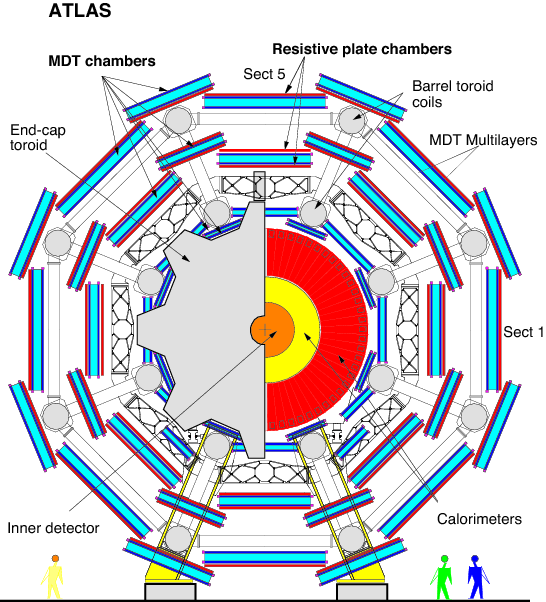
\includegraphics[width=0.8\textwidth]{chapters/c4/figures/mu-bar}
  \caption{a}
  \label{fig:mu-bar}
\end{subfigure}%
\begin{subfigure}{.5\textwidth}
  \centering
    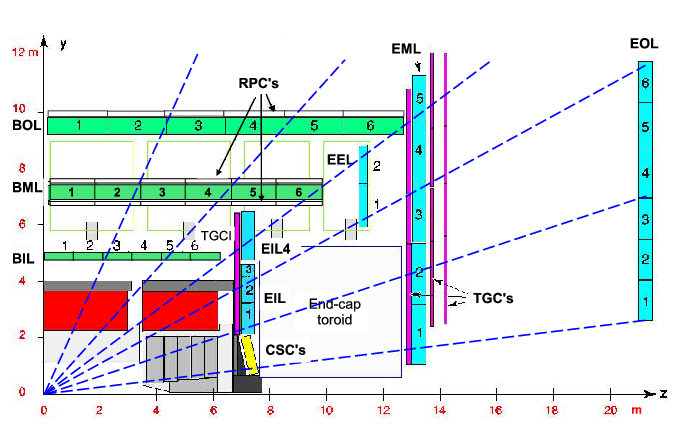
\includegraphics[width=0.8\textwidth]{chapters/c4/figures/mu-end}
  \caption{b}
  \label{fig:mu-end}
\end{subfigure}
    \caption{Geometric layout of muon sub-detectors in barrel (\ref{fig:mu-bar}) and end-cap (\ref{fig:mu-end) region}
\label{fig:mu}
\end{figure}
Sample text sample text sample text. Sample text sample text sample text.
Sample text sample text sample text. Sample text sample text sample text.
Sample text sample text sample text. Sample text sample text sample text.

\section{Muon Spectrometer}
\label{sec:for}
Sample text sample text sample text. Sample text sample text sample text.
Sample text sample text sample text. Sample text sample text sample text.
Sample text sample text sample text. Sample text sample text sample text.

\subsection{Thin Gap Chambers}
Sample text sample text sample text. Sample text sample text sample text.
\section{Event simulation}
Sample text sample text sample text. Sample text sample text sample text.
Sample text sample text sample text. Sample text sample text sample text.
Sample text sample text sample text. Sample text sample text sample text.

\section{Event generator}
\label{sec:data}
Sample text sample text sample text. Sample text sample text sample text.
Sample text sample text sample text. Sample text sample text sample text.
Sample text sample text sample text. Sample text sample text sample text.

\section{Detector simulation}
Sample text sample text sample text. Sample text sample text sample text.
Sample text sample text sample text. Sample text sample text sample text.
Sample text sample text sample text. Sample text sample text sample text.
